

\documentclass[journal]{IEEEtran}
%
% If IEEEtran.cls has not been installed into the LaTeX system files,
% manually specify the path to it like:
% \documentclass[journal]{../sty/IEEEtran}

% 加入对中文的支持
\usepackage{ctex}			% 假如不需要中文,把这一行删了就行
\usepackage{graphicx} 		% 图形支持
%\RequirePackage{graphicx} 	% 图形
\graphicspath{{figures/}} 	% 修改图片文件路径
\usepackage{amsmath} 		% 公式支持
\usepackage{array} 			% 部分表格支持

\hyphenation{op-tical net-works semi-conduc-tor}


\begin{document}
%
% paper title
% Titles are generally capitalized except for words such as a, an, and, as,
% at, but, by, for, in, nor, of, on, or, the, to and up, which are usually
% not capitalized unless they are the first or last word of the title.
% Linebreaks \\ can be used within to get better formatting as desired.
% Do not put math or special symbols in the title.
\title{99\%高效隔离三相矩阵型DAB降压-升压功率因数校正整流器}
%
%
% author names and IEEE memberships
% note positions of commas and nonbreaking spaces ( ~ ) LaTeX will not break
% a structure at a ~ so this keeps an author's name from being broken across
% two lines.
% use \thanks{} to gain access to the first footnote area
% a separate \thanks must be used for each paragraph as LaTeX2e's \thanks
% was not built to handle multiple paragraphs
%

\author{Lukas ~Schrittwieser,~\IEEEmembership{Member,~IEEE,}
Michael~Leibl,~\IEEEmembership{Member,~IEEE,}
and~Johann~W. Kolar,~\IEEEmembership{Fellow,~IEEE} }
%  \  翻译(初稿):中南大学 \ 电气17陈宝轩 \ 2021.02.11 

%\thanks{稿件收到2018年10月28日;2019年2月13日修订;2019年4月14日接受。出版日期2019年5月1日;当前版本日期2019年10月14日。由副主编D. Xu.推荐出版。(对应作者:Lukas Schrittwieser)}% <-this % stops a space
%
%\thanks{L. Schrittwieser在瑞士苏黎世联邦理工学院电力电子系统实验室工作,邮编:8092。他现在在瑞士营养品with Technokrat GmbH工作(电子邮件:ls@technokrat.ch)}
%
%\thanks{米(meter的缩写))莱博在瑞士苏黎世联邦理工学院电力电子系统实验室工作,邮编:8092。他现在在瑞士森瓦尔德9466号Brusa Elektronik AG工作(电子邮件:michael.leibl@icloud.com)}
%
%\thanks{J.W. Kolar在瑞士苏黎世联邦理工学院电力电子系统实验室工作(电子邮件:kolar@lem.ee.ethz.ch)}
%
%\thanks{本文中一个或多个图形的彩色版本可在http://ieeexplore.ieee.org在线获得。}% <-this % stops a space
%
%\thanks{数字对象识别器10.1109/TPEL . 2019 . 291448888816} }

% note the % following the last \IEEEmembership and also \thanks - 
% these prevent an unwanted space from occurring between the last author name
% and the end of the author line. i.e., if you had this:
% 
% \author{....lastname \thanks{...} \thanks{...} }
% ^------------^------------^----Do not want these spaces!
%
% a space would be appended to the last name and could cause every name on that
% line to be shifted left slightly. This is one of those "LaTeX things". For
% instance, "\textbf{A} \textbf{B}" will typeset as "A B" not "AB". To get
% "AB" then you have to do: "\textbf{A}\textbf{B}"
% \thanks is no different in this regard, so shield the last } of each \thanks
% that ends a line with a % and do not let a space in before the next \thanks.
% Spaces after \IEEEmembership other than the last one are OK (and needed) as
% you are supposed to have spaces between the names. For what it is worth,
% this is a minor point as most people would not even notice if the said evil
% space somehow managed to creep in.



% The paper headers
\markboth{ IEEE TRANSACTIONS ON POWER ELECTRONICS,~VOL.~35, NO.~1, JANUARY~2020}%
{SCHRITTWIESER et al.: 99\% EFFICIENT ISOLA TED THREE-PHASE MA TRIX-TYPE DAB BUCK–BOOST PFC RECTIFIER}
%{Shell \MakeLowercase{\textit{et al.}}: Bare Demo of IEEEtran.cls for IEEE Journals}
% The only time the second header will appear is for the odd numbered pages
% after the title page when using the twoside option.
% 
% *** Note that you probably will NOT want to include the author's ***
% *** name in the headers of peer review papers. ***
% You can use \ifCLASSOPTIONpeerreview for conditional compilation here if
% you desire.




% If you want to put a publisher's ID mark on the page you can do it like
% this:
%\IEEEpubid{0000--0000/00\$00.00~\copyright~2015 IEEE}
% Remember, if you use this you must call \IEEEpubidadjcol in the second
% column for its text to clear the IEEEpubid mark.



% use for special paper notices
%\IEEEspecialpapernotice{(Invited Paper)}




% make the title area
\maketitle

% As a general rule, do not put math, special symbols or citations
% in the abstract or keywords.
\begin{abstract}

三相功率因数校正整流器是电力电子的一个重要领域,它从公共三相电源向直流负载提供几十千瓦或更多的功率,并实现电流的正弦输入。在许多应用中,例如为了确保安全或出于不同的接地方案等原因,电源和负载之间需要进行隔离。本文介绍了一种降压-升压型、单位功率因数、隔离矩阵型、双有源桥三相整流器的调制、设计和实现。它使用了一个与传统的双有源桥相似的电路,但采用直接矩阵变换器将高频变压器的初级绕组和电源相连。提出并综合分析了一种软开关调制方案,导出了闭合形式的解和数值优化问题,以计算实现最小传导损耗的开关时间。在此分析的基础上,讨论了 8-kW 400V有效值的三相交流至400V直流样机的设计,力求实现最高的效率。我们使用900V的 碳化硅MOSFETS和一个有集成电感的变压器,功率密度可达$4kW \cdot dm^{-3}(66 W \cdot in^{-3})$。测量结果表明,标称工作条件下的超高全功率效率为99.0\%,输入电压低10\%时为98.7\%。

\end{abstract}

% Note that keywords are not normally used for peerreview papers.
\begin{IEEEkeywords}
直接矩阵型, 双有源桥, 隔离型整流器, 三相功率因数校正转换器.
\end{IEEEkeywords}






% For peer review papers, you can put extra information on the cover
% page as needed:
% \ifCLASSOPTIONpeerreview
% \begin{center} \bfseries EDICS Category: 3-BBND \end{center}
% \fi
%
% For peerreview papers, this IEEEtran command inserts a page break and
% creates the second title. It will be ignored for other modes.
\IEEEpeerreviewmaketitle



\section{绪论}
% The very first letter is a 2 line initial drop letter followed
% by the rest of the first word in caps.
% 
% form to use if the first word consists of a single letter:
% \IEEEPARstart{A}{demo} file is ....
% 
% form to use if you need the single drop letter followed by
% normal text (unknown if ever used by the IEEE):
% \IEEEPARstart{A}{}demo file is ....
% 
% Some journals put the first two words in caps:
% \IEEEPARstart{T}{his demo} file is ....
% 
% Here we have the typical use of a "T" for an initial drop letter
% and "HIS" in caps to complete the first word.
近年来,住宅区和商业或办公建筑中固有直流(dc)负载的数量和功率需求显著增加。这些负载包括电动汽车、LED照明、节能空调和通风系统的变速驱动器以及信息和通信技术设备,如台式计算机、服务器和数据中心。同时,作为可再生能源,如光伏板和小型风力涡轮机,产生的直流电的数量也在增加。因此,仅跨越单个商业建筑、工业厂房或整个住宅区的直流配电系统有望降低转换损耗、提高可靠性和/或降低成本。这些被称作直流微电网的在科学文献、研究和工业中受到了极大的关注[1]–[4]。


\section{调制}

\subsection{ZVS/ZCS开关模式}

\vspace*{-1em} % 间距减小行数
\begin{gather} % 不要序号显示\begin{gather*}...\end{gather*}
u_p(t)=
\begin{cases}
	u_{ac},& {0\leq t < \frac{1}{2} -t_2}\\
	u_{ab},& {\frac{1}{2} -t_2 \leq t < \frac{1}{2} -t_1 }\\
	0,& {\frac{1}{2} -t_1 \leq t < \frac{1}{2}}\\
	-u_p(t-\frac{1}{2}),& {\frac{1}{2} \leq t_1 < 1}
	\end{cases}
\end{gather}

\subsection{传导损耗最佳功率因数校正(FPC)调制}

从图1(b)所示的整流器原理图中可以看出,变压器的一次侧绕组电流$i_p$是由DMC的四个MOSFET传导,而与DMC的导通状态无关。

\subsubsection{不连续传导模式(DCM)}

aaaaaa

\subsubsection{连续传导模式(DCM)}

bbbbb


\begin{figure}[h]
\centering
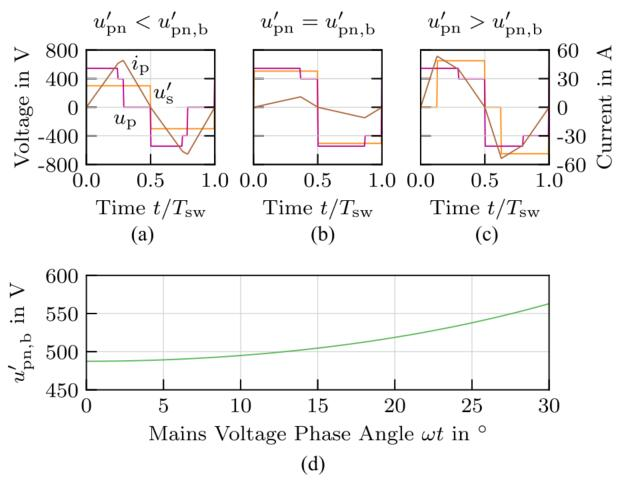
\includegraphics[width=3.6in]{fig7.jpg} % scale=0.6
\caption{$\omega t = 15^\circ$的变压器电压和变压器电流,工作在DCM模式下的最大可能输出电流$i_{dc,DCM,max}$。在(a)中,输出电压$u'_{pn}= 300 V$低于边界值$u'_{p,n.b}= 505 V$,因此,$u'_s$的占空比是最大的,$u_p$和$u'_s$的上升沿对齐。(b)当案例$u'_{pn}= u'_{pn,b}$时,$u_p$和$u'_s$都使用最大可能的占空比。(c) 当$u'_{pn}=650V > u'_{pn,b}$时,只有$u_p$的占空比最大,$u_p$和$u'_s$的下降沿对齐。(d),当标称输入电压(相电压)的有效值$U_1= 230$时,$u'_{pn,b}$关于电源电压相角$\omega t$的函数图像。}
\label{fig7}
\end{figure}

\begin{table}[h]
\caption{标称工作条件和转换器规格}
\label{table1}
\centering
\begin{tabular}{ll}
\hline
Input Voltage (Line-to-Neutral) & $U_1 = 230 V rms$\\
Input Frequency & $w=2\pi50Hz$\\
Nominal DC Output Voltage & $U_{pn}=400V$\\
Nominal Output Power & $P=8kW$\\
Nominal Swithing Frequency & $f_{sw} = 31 kHz$\\
Leakage Inductance & $L_1=36uH$\\
Turns Ratio & $n_p/n_s = 22/17\approx 1.29$\\
\hline
\end{tabular}
\end{table}

\subsection{变压器波形}

对于四种不同的电源电压相角$\omega t$,测量的变压器电压$u_p$和$u_s$相应的绕组电流$i_p$如图22所示。这些图是在标称工作条件下记录的,负载电流为20 A,如表1所示。可以看出,初级侧绕组电压的下降沿和次级侧电压的上升沿完全发生在绕组电流$i_p$和$i_s$为正的情况下,这意味着实现了完全的ZVS。


\begin{table*}[h]
\caption{与其他隔离型三相功率因数校正整流器的比较}
\label{table2}
\centering
\begin{tabular}{cccccc}
\hline
Topology & Technology & Rated Power & DC voltage & Meas. Efficiency & Power Density \\
\hline
Phase-Modular SEPIC [43] & Si IGBT \& Si Diodes & 4 kW & 400 V & 90 \% & unknown \\
Isolated Full-Bridge Boost [44] & Si IGBT & 1.7kW & 200 V & 91 \% & unknown \\
Swiss-Forward [21] & SiC MOSFET \& SiC Schottky & 3 kW & 270 V & 93.5 \% & 0.44 kW $dm^{-3}$ \\
Matrix-Type Isolated Inverter [45] & SiC MOSFET & 1.3 kW & 400 V & 94.1\% & unknown \\
IMDAB3R [46] & SiC MOSFET \& SiC Schottky & 1.2 kW & 180 V & 94.4 \% & unknown \\
Phase-Modular \& Scott Transformer [47] & Si IGBT \& Si Diode & 12 kW & 400V & 95.1 \% & 1.33 kW $dm^{-3}$ \\
Phase-Modular Cuk [48] & SiC MOSFET \& Si Diode & 2 kW & 400 V & 95.1 \% & unknown \\
Phase-Modular PFC \& LLC [49] & Si MOSFET \& SiC Diode & 10kW & 300 V & 95.5 \% & unknown \\
IMDAB3R [14] & SiC MOSFET & 1 kW & 230 V & 96.0 \% & unknown\\
Isolated Matrix-Type $\triangle$ Rectifier [50] & SiC MOSFET \& SiC Schottky & 7.5 kW & 400 V & 97.2 \% & 1.03 kW $dm^{-3}$ \\
Phase-Modular PFC \& LLC [51] & GaN HEMT & 22 kW & 400 V & 98 \% & 3.3kW $dm^{-3}$ \\
\hline
This Work & SiC MOSFET & 8kW & 400 V & 99.0\% & 4.0kW $dm^{-3}$ \\
\hline
\end{tabular}
\end{table*}

%\section{输入和输出电流的计算}
%\subsection{AAA}
%\subsubsection{aaa}


% An example of a floating figure using the graphicx package.
% Note that \label must occur AFTER (or within) \caption.
% For figures, \caption should occur after the \includegraphics.
% Note that IEEEtran v1.7 and later has special internal code that
% is designed to preserve the operation of \label within \caption
% even when the captionsoff option is in effect. However, because
% of issues like this, it may be the safest practice to put all your
% \label just after \caption rather than within \caption{}.
%
% Reminder: the "draftcls" or "draftclsnofoot", not "draft", class
% option should be used if it is desired that the figures are to be
% displayed while in draft mode.
%


% Note that the IEEE typically puts floats only at the top, even when this
% results in a large percentage of a column being occupied by floats.


% An example of a double column floating figure using two subfigures.
% (The subfig.sty package must be loaded for this to work.)
% The subfigure \label commands are set within each subfloat command,
% and the \label for the overall figure must come after \caption.
% \hfil is used as a separator to get equal spacing.
% Watch out that the combined width of all the subfigures on a 
% line do not exceed the text width or a line break will occur.
%
%\begin{figure*}[!t]
%\centering
%\subfloat[Case I]{\includegraphics[width=2.5in]{box}%
%\label{fig_first_case}}
%\hfil
%\subfloat[Case II]{\includegraphics[width=2.5in]{box}%
%\label{fig_second_case}}
%\caption{Simulation results for the network.}
%\label{fig_sim}
%\end{figure*}
%
% Note that often IEEE papers with subfigures do not employ subfigure
% captions (using the optional argument to \subfloat[]), but instead will
% reference/describe all of them (a), (b), etc., within the main caption.
% Be aware that for subfig.sty to generate the (a), (b), etc., subfigure
% labels, the optional argument to \subfloat must be present. If a
% subcaption is not desired, just leave its contents blank,
% e.g., \subfloat[].


% An example of a floating table. Note that, for IEEE style tables, the
% \caption command should come BEFORE the table and, given that table
% captions serve much like titles, are usually capitalized except for words
% such as a, an, and, as, at, but, by, for, in, nor, of, on, or, the, to
% and up, which are usually not capitalized unless they are the first or
% last word of the caption. Table text will default to \footnotesize as
% the IEEE normally uses this smaller font for tables.
% The \label must come after \caption as always.
%
%\begin{table}[!t]
%% increase table row spacing, adjust to taste
%\renewcommand{\arraystretch}{1.3}
% if using array.sty, it might be a good idea to tweak the value of
% \extrarowheight as needed to properly center the text within the cells
%\caption{An Example of a Table}
%\label{table_example}
%\centering
%% Some packages, such as MDW tools, offer better commands for making tables
%% than the plain LaTeX2e tabular which is used here.
%\begin{tabular}{|c||c|}
%\hline
%One & Two\\
%\hline
%Three & Four\\
%\hline
%\end{tabular}
%\end{table}


% Note that the IEEE does not put floats in the very first column
% - or typically anywhere on the first page for that matter. Also,
% in-text middle ("here") positioning is typically not used, but it
% is allowed and encouraged for Computer Society conferences (but
% not Computer Society journals). Most IEEE journals/conferences use
% top floats exclusively. 
% Note that, LaTeX2e, unlike IEEE journals/conferences, places
% footnotes above bottom floats. This can be corrected via the
% \fnbelowfloat command of the stfloats package.


\section{总结和结论}

本文分析了IMDAB3R,它最初是作为车辆到电网的接口提出的。由于其结构类似于传统的DAB转换器,具有足够大的漏电感的隔离变压器是除EMI滤波器之外唯一需要的磁性元件。这简化了机械设计,并潜在地降低了成本和/或体积。此外,IMDAB3R不需要任何电流传感器,因为通过变压器电流的开环控制,可以获得令人满意的3\%电源输入电流THD值。


% if have a single appendix:
%\appendix[Proof of the Zonklar Equations]
% or
%\appendix % for no appendix heading
% do not use \section anymore after \appendix, only \section*
% is possibly needed

% use appendices with more than one appendix
% then use \section to start each appendix
% you must declare a \section before using any
% \subsection or using \label (\appendices by itself
% starts a section numbered zero.)
%


\appendices
\section{市电输入电流的方程式推导}


啦啦啦啦啦

\vspace*{-1em} 
\begin{align}
\xi (0) = & \ \xi \biggr(\frac{1}{2}\biggr)=\xi(1)=0 \\
\xi \biggr(t+\frac{1}{2}\biggr) = & - \xi(t).
\end{align}




% you can choose not to have a title for an appendix
% if you want by leaving the argument blank
%\section{}
%Appendix two text goes here.


% use section* for acknowledgment
\section*{感谢}

作者要感谢E. L. Barrios博士分享了他在极低损耗变压器方面的知识,并帮助设计和测试了一个初始原型机。


% Can use something like this to put references on a page
% by themselves when using endfloat and the captionsoff option.
\ifCLASSOPTIONcaptionsoff
\newpage
\fi



% trigger a \newpage just before the given reference
% number - used to balance the columns on the last page
% adjust value as needed - may need to be readjusted if
% the document is modified later
%\IEEEtriggeratref{8}
% The "triggered" command can be changed if desired:
%\IEEEtriggercmd{\enlargethispage{-5in}}

% references section

% can use a bibliography generated by BibTeX as a .bbl file
% BibTeX documentation can be easily obtained at:
% http://mirror.ctan.org/biblio/bibtex/contrib/doc/
% The IEEEtran BibTeX style support page is at:
% http://www.michaelshell.org/tex/ieeetran/bibtex/

% 这里可以使用事先定义好了的IEEE参考文献目录
%\bibliographystyle{IEEEtran}
% argument is your BibTeX string definitions and bibliography database(s)
%\bibliography{IEEEabrv,../bib/paper}
%
% <OR> manually copy in the resultant .bbl file
% set second argument of \begin to the number of references
% (used to reserve space for the reference number labels box)
\begin{thebibliography}{1}

\bibitem{IEEEhowto:kopka}
T. Dragiˇ cevi´ c, X. Lu, J. C. V asquez, and J. M. Guerrero, “DC microgrids—
Part II: A review of power architectures, applications and standardization issues,” IEEE Trans. Power Electron., vol. 31, no. 5, pp. 3528–3549,May 2016.

\bibitem{IEEEhowto:kopka}
M. Noritake, K. Y uasa, T. Takeda, H. Hoshi, and K. Hirose, “Demonstrative research on DC microgrids for office buildings,” in Proc. IEEE Int.Telecommun. Energy Conf., Sep. 2014, pp. 1–5.

\bibitem{IEEEhowto:kopka}
D. J. Becker and B. J. Sonnenberg, “DC microgrids in buildings and data centers,” in Proc. IEEE Int. Telecommun. Energy Conf., Oct. 2011,pp. 1–7.

\bibitem{IEEEhowto:kopka}
H. Kakigano, Y . Miura, and T. Ise, “Low-voltage bipolar-type DC microgrid for super high quality distribution,” IEEE Trans. Power Electron., vol. 25, no. 12, pp. 3066–3075, Dec. 2010.


\end{thebibliography}



% biography section
% 
% If you have an EPS/PDF photo (graphicx package needed) extra braces are
% needed around the contents of the optional argument to biography to prevent
% the LaTeX parser from getting confused when it sees the complicated
% \includegraphics command within an optional argument. (You could create
% your own custom macro containing the \includegraphics command to make things
% simpler here.)
%\begin{IEEEbiography}[{\includegraphics[width=1in,height=1.25in,clip,keepaspectratio]{mshell}}]{Michael Shell}
% or if you just want to reserve a space for a photo:

\begin{IEEEbiography}[{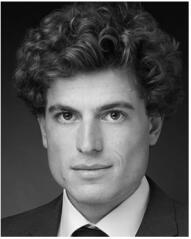
\includegraphics[width=1in,height=1.25in,clip,keepaspectratio]{Michael}}]{Michael Leibl}

2010年在奥地利维也纳的维也纳理工大学获得学士学位,2012年在瑞士苏黎世的瑞士联邦理工学院获得硕士学位,均为电气工程专业。

他目前在瑞士森瓦尔德的布鲁萨电子公司工作。直到2017年,他一直在电力电子系统实验室撰写关于三相整流器和x光系统高压电源的博士论文,涵盖了他的主要研究兴趣,包括电感元件的优化设计,特别是高频绕组损耗建模、大功率三相功率因数校正整流器和隔离直流-直流转换器。
\end{IEEEbiography}

\begin{IEEEbiography}[{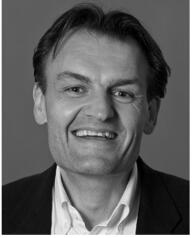
\includegraphics[width=1in,height=1.25in,clip,keepaspectratio]{Johann}}]{Johann W. Kolar}

(10)分别于1997年和1999年在奥地利维也纳的维也纳理工大学获得硕士和博士学位。

自1984年以来,他一直与维也纳理工大学密切合作,在电力电子、工业电子和高性能驱动系统领域担任独立研究员和国际顾问。他提出了许多新颖的脉宽调制转换器拓扑、调制和控制概念,并指导了70多名博士生。他在国际期刊和会议记录中撰写或合著了880多篇科学论文,四本书的章节,并申请了190多项专利。他目前的研究重点是超紧凑和超高效的SicAndGanConverters系统、固态变压器、先进的变速三相电机驱动、集成模块化电机驱动、超高速电机、无轴承电机/执行器以及电力电子/机电一体化设计自动化。

\\

中南大学

电气1705陈宝轩 

翻译

2021.02.11(初稿)

\end{IEEEbiography}
%
%% if you will not have a photo at all:
%\begin{IEEEbiographynophoto}{John Doe}
%Biography text here.
%\end{IEEEbiographynophoto}

% insert where needed to balance the two columns on the last page with
% biographies
%\newpage

%\begin{IEEEbiographynophoto}{Jane Doe}
%Biography text here.
%\end{IEEEbiographynophoto}

% You can push biographies down or up by placing
% a \vfill before or after them. The appropriate
% use of \vfill depends on what kind of text is
% on the last page and whether or not the columns
% are being equalized.

%\vfill

% Can be used to pull up biographies so that the bottom of the last one
% is flush with the other column.
%\enlargethispage{-5in}



% that's all folks
\end{document}



